\documentclass[14pt, a4paper]{extarticle}
\usepackage{GOST}
\usepackage{array}
\usepackage{verbatim}
\usepackage[detect-all]{siunitx}
\usepackage{amsmath}
\usepackage{amssymb}
\usepackage[utf8]{inputenc}
\usepackage{hyperref}
\usepackage{tempora}

\makeatletter
\renewcommand\@biblabel[1]{#1.}
\makeatother

\usepackage{listings}
\lstset{ 
	language=[Sharp]C,                 % выбор языка для подсветки (здесь это С)
	%basicstyle=\small\sffamily, % размер и начертание шрифта для подсветки кода
	keywordstyle=\color{blue}\textbf,
	numberstyle=\scriptsize\color{gray},
	numbers=left,               % где поставить нумерацию строк (слева\справа)
	numberstyle=\tiny,           % размер шрифта для номеров строк
	stepnumber=1,                   % размер шага между двумя номерами строк
	numbersep=5pt,                % как далеко отстоят номера строк от подсвечиваемого кода
	showspaces=false,            % показывать или нет пробелы специальными отступами
	showstringspaces=false,      % показывать или нет пробелы в строках
	showtabs=false,             % показывать или нет табуляцию в строках
	frame=single,              % рисовать рамку вокруг кода
	tabsize=2,                 % размер табуляции по умолчанию равен 2 пробелам
	captionpos=t,              % позиция заголовка вверху [t] или внизу [b] 
	breaklines=true,           % автоматически переносить строки (да\нет)
	breakatwhitespace=false, % переносить строки только если есть пробел
}


\usepackage{pgfplots}
\usepackage{filecontents}
\usetikzlibrary{datavisualization}
\usetikzlibrary{datavisualization.formats.functions}

\begin{document}
	
\begin{table}[ht]
	\centering
	\begin{tabular}{|c|p{400pt}|} 
		\hline
		\begin{tabular}[c]{@{}c@{}} 
\includegraphics[scale=1]{source/b_logo.jpg} \\\end{tabular} &
		\footnotesize\begin{tabular}[c]{@{}c@{}}\textbf{Министерство~науки~и~высшего~образования~Российской~Федерации}\\\textbf{Федеральное~государственное~бюджетное~образовательное~учреждение}\\\textbf{~высшего~образования}\\\textbf{«Московский~государственный~технический~университет}\\\textbf{имени~Н.Э.~Баумана}\\\textbf{(национальный~исследовательский~университет)»}\\\textbf{(МГТУ~им.~Н.Э.~Баумана)}\\\end{tabular}  \\
		\hline
	\end{tabular}
\end{table}
\noindent\rule{\textwidth}{4pt}
\noindent\rule[14pt]{\textwidth}{1pt}
\hfill 
\noindent
\makebox{ФАКУЛЬТЕТ~}%
\makebox[\textwidth][l]{\underline{~«Информатика и системы управления»~~~~~~~~~~~~~~~~~~~~~~~~~~~~~~~~~}}%
\\
\noindent
\makebox{КАФЕДРА~}%
\makebox[\textwidth][l]{\underline{~«Программное обеспечение ЭВМ и информационные технологии»~}}%
\\

\begin{center}
	\vspace{1.5cm}
	{\bf\huge Отчёт\par}
	{\bf\Large по лабораторной работе № 5\par}
	\vspace{0.7cm}
\end{center}
 
\noindent
\makebox{\large{\bf Название:}~~~}
\makebox[\textwidth][l]{\large\underline{~Многопоточная реализация конвейера~}}\\

\noindent
\makebox{\large{\bf Дисциплина:}~~~}
\makebox[\textwidth][l]{\large\underline{~Анализ алгоритмов}}\\

\vspace{1.5cm}
\noindent
\begin{tabular}{l c c c c c}
	Студент      & ~ИУ7-55Б~               & \hspace{2.5cm} & \hspace{2cm}                 & &  Д.О. Склифасовский \\\cline{2-2}\cline{4-4} \cline{6-6} 
	\hspace{3cm} & {\footnotesize(Группа)} &                & {\footnotesize(Подпись, дата)} & & {\footnotesize(И.О. Фамилия)}
\end{tabular}

\noindent
\begin{tabular}{l c c c c}
	Преподователь & \hspace{5cm}   & \hspace{2cm}                 & & ~~~~~~Л.Л. Волкова~~~~~~\\\cline{3-3} \cline{5-5} 
	\hspace{3cm}  &                & {\footnotesize(Подпись, дата)} & & {\footnotesize(И.О. Фамилия)}
\end{tabular}

\vspace{0.6cm}
\begin{center}	
	\vfill
	\large \textit {Москва, 2020}
\end{center}

\thispagestyle {empty}
\pagebreak

% СОДЕРЖАНИЕ 
\clearpage
\tableofcontents

% ВВЕДЕНИЕ
\clearpage
\section*{Введение}
\addcontentsline{toc}{section}{Введение}
Цель работы: создать систему конвейерной обработки.\par
В ходе лабораторной работы требуется:
\begin{enumerate}
	\item[1)] описать алгоритм, реализующий конвейерную обработку;
	\item[2)] реализовать данный алгоритм;
	\item[3)] провести тестирование алгоритма.
\end{enumerate}\par

% АНАЛИТИЧЕСКИЙ РАЗДЕЛ
\clearpage
\section{Аналитический раздел}
В данном разделе представлены принципы конвейерной обработки и параллельных вычислений.
\subsection{Общие сведения}
Ленточный \textbf{конвейер} (англ. belt conveyor) — транспортирующее устройство непрерывного действия с рабочим органом в виде ленты. \par
\textbf{Конвейерное производство} – это разновидность организации современного производственного процесса \hyperref[literature]{[1]}. Конвейер используется повсеместно. Он облегчил труд человека и повысил производительность. С его помощью к процессу изготовления продукции задействуют минимальное количество сотрудников. Такое оборудование позволяет будущему товару, самостоятельно проходить различные стадии производства. С его появлением, компании смогли повысить свои показатели, изготавливая конечную продукцию в разы быстрее.
\subsection{Параллельное программирование}
Параллельное программирование. Параллельное программирование служит для создания программ, эффективно использующих вычислительные ресурсы за счет одновременного исполнения кода на нескольких вычислительных узлах. Для создания параллельных приложений используются параллельные языки программирования и специализированные системы поддержки параллельного программирования, такие как MPI и OpenMP. Параллельное программирование является более сложным по сравнению с последовательным как в написании кода, так и в его отладки. Для облегчения процесса параллельного программирования существуют специализированные инструменты, например, отладчик TotalView.\hyperref[literature]{[2]}
\subsection{Вывод}
В данном разделе были рассмотрены основы конвейерной обработки и технология параллельного программирования.
\clearpage
\section{Конструкторский раздел}
В данном разделе представлена схема алгоритмов обработки элементов линии конвейера.
\subsection{Разработка алгоритма}
На \hyperref[Algorithm1]{рисунке 1} изображена схема алгоритма запуска линии конвейера.
\begin{figure}[h!]\label{Algorithm1}
	\center{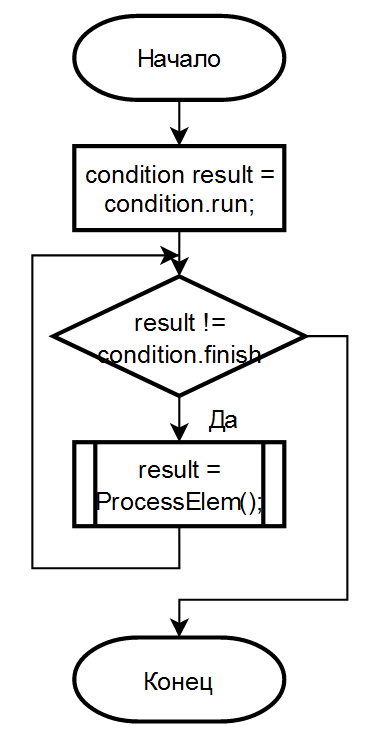
\includegraphics[scale=0.8]{source/RunLine.png}}
	\caption{Схема алгоритма запуска линии конвейера}
\end{figure}
\clearpage
На \hyperref[Algorithm2]{рисунке 2} изображена схема алгоритма обработка элементов линии.
\begin{figure}[h!]\label{Algorithm2}
	\center{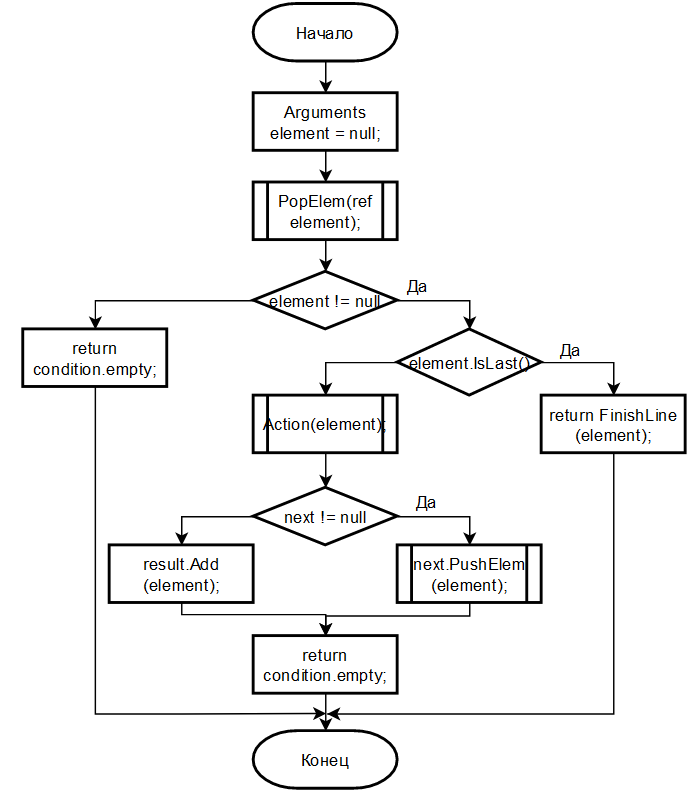
\includegraphics[scale=0.9]{source/ProcessElem.png}}
	\caption{Схема алгоритма обработка элементов линии}
\end{figure}
\subsection{Описание системы}
Система состоит из трех линий (очередей), который последовательно соединены между собой (у каждой линии есть ссылка на следующую). Изначально генерируются аргументы. У последнего из аргументов присутствует флаг, указывающий на то, что он последний. Все аргументы записываются в первую очередь, а из последней попадают в результирующий массив. Выдается время начала и конца обработки элемента.
\subsection{Вывод}
В данном разделе были рассмотрены схема алгоритмов обработки элементов линии конвейера и описана система ПО.
\clearpage
\section{Технологический раздел}
В данном разделе даны общие требования к программе, средства реализации и сама реализация алгоритмов.
\subsection{Общие требования}
\textbf{Требования к программе}
\begin{enumerate}
	\item[1)] аргументы должны последовательно проходить линии в заданном порядке;
	\item[2)] каждая линия должна работать в своем потоке;
	\item[3)] последним элементом должен быть флаг, при поступлении которого, линия должна завершить свою работу;
	\item[4)] при пустой очереди линии, она должна ожидать поступления нового элемента;
	\item[5)] в результате из последней линии должен вернуться массив аргументов, у которого порядок совпадает с начальным.
\end{enumerate}
\subsection{Средства реализации}
В качестве языка программирования был выбран C\#, так как я знаком с данным языком программирования, имею представление о способах тестирования программы.\hyperref[literature]{[3]}\par
Средой разработки Visual Studio.\hyperref[literature]{[4]}\par 
Для замеров процессорного времени используется функция $Stopwatch$.\hyperref[literature]{[5]}\hyperref[literature]{[6]}\par
Многопоточное программирование было реализовано с помощью пространства имен System.Threading.\hyperref[literature]{[7]}
\subsection{Сведения о модулях программы}
Программа состоит из:
\begin{enumerate}
	\item[1)] Program.cs - главный файл программы, в котором располагается точка входа в программу;
	\item[2)] Arguments.cs - файл класса Arguments;
	\item[3)] Line.cs - файл класса линии конвейера;
\end{enumerate}
\subsection{Листинг кода программы}
В листинге 1 реализован алгоритм запуска линии конвейера.
\begin{lstlisting}[label=RunLine, caption=Запуска линии конвейера]
public void RunLine()
{
	condition result = condition.run;
	while (result != condition.finish)
	{
		result = ProcessElem();
	}
}
\end{lstlisting}
В листинге 2 реализован алгоритм обработки аргумента линии.
\begin{lstlisting}[label=RunLine, caption=Обработки аргумента линии]
private condition ProcessElem()
{
	Arguments element = null;
	PopElem(ref element);
	if (element != null)
	{
		if (element.IsLast())
		{
			return FinishLine(element);
		}
		Action(element);
		if (next != null)
		{
			next.PushElem(element);
		}
		else if (isLast)
		{
			result.Add(element);
		}
	}
	else
	{
		return condition.empty;
	}
	return condition.run;
}
\end{lstlisting}
В листинге 3 реализовано добавление элемента в очередь.
\begin{lstlisting}[label=PushElem, caption=Добавление элемента в очередь]
public void PushElem(Arguments arg)
{
	lock(myQueue)
	{
		myQueue.Enqueue(arg);
	}
}
\end{lstlisting}
В листинге 4 реализовано взятие элемента из очереди.
\begin{lstlisting}[label=PopElem, caption=Взятие элемента из очеред]
private void PopElem(ref Arguments arg)
{
	lock (myQueue)
	{
		if (myQueue.Count > 0)
		{
			arg = myQueue.Dequeue();
		}
	}
}
\end{lstlisting}
\subsection{Вывод}
В данном разделе были даны общие требования к программе, описаны средства реализации, были представлены сведения о модулях программы, а также реализованы алгоритмы работы линии конвейера.
\clearpage
\section{Экспериментальный раздел}
В данном разделе представлен результаты работы программы и показано параллельное выполнение операций.
\subsection{Пример работы программы}
На \hyperref[result]{рисунке 3} изображена результат работы программы.
\begin{figure}[h!]\label{result}
	\center{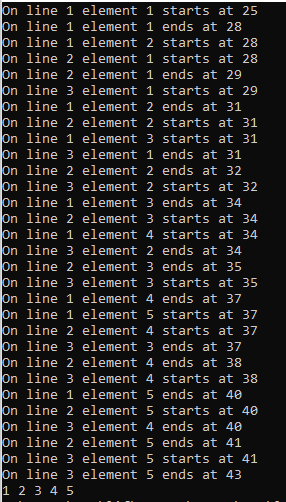
\includegraphics[scale=0.9]{source/result.png}}
	\caption{Результат работы программы}
\end{figure}
\subsection{Вывод}
Результаты работы программы показывают, что действия, а именно начало обработки элементов и конец, выполнялись не последовательно, а каждая линия работала параллельно. Конечный результат показывает, что последовательность элементов сохраняется.
\clearpage
\section{Заключение}
В ходе выполнения лабораторной работы были изучены возможности параллельных вычислений и был использован такой подход на практике. Был разработан конвейер с параллельно работающими линиями. Конвейерная обработка позволяет ускорить работу программы, если требуется обработка однотипных данных.
\clearpage
\section*{Литература}
\addcontentsline{toc}{section}{Литература}
\begin{enumerate}
	\label{literature}
	\item Конвейерное производство. -URL: \href{http://dirsystem.ru/konvejernoe-proizvodstvo}{http://dirsystem.ru/konvejernoe-proizvodstvo} (дата обращения 19.11.2020). -Текст: электронный.
	\item Параллельное программирование. -URL: \href{https://www.viva64.com/ru/t/0038/}{https://www.viva64.com/ru/t/0038/} (дата обращения: 24.10.2020). -Текст: электронный.
	\item  Документация по C\#. -URL: \href{https://docs.microsoft.com/ru-ru/dotnet/csharp/}{https://docs.microsoft.com/ru-ru/dotnet/csharp/} (дата обращения: 24.10.2020). -Текст: электронный.
	\item Документация по семейству продуктов Visual Studio. -URL:\par \href{https://docs.microsoft.com/ru-ru/visualstudio/?view=vs-2019}{https://docs.microsoft.com/ru-ru/visualstudio/?view=vs-2019 } (дата обращения: 01.10.2020). -Текст: электронный.
	\item Stopwatch Класс. -URL: \href{https://goo.su/2e99}{https://goo.su/2e99 } (дата обращения: 24.10.2020). -Текст: электронный.
	\item Под капотом у Stopwatch. -URL:  \href{https://habr.com/ru/post/226279/}{https://habr.com/ru/post/226279/} (дата обращения: 24.10.2020). Текст: электронный.
	\item Thread Класс. -URL:  \href{https://docs.microsoft.com/ru-ru/dotnet/api/system.threading.thread?view=net-5.0}{https://docs.microsoft.com/ru-ru/dotnet/api/system.threading.thread?view=net-5.0} (дата обращения: 19.11.2020). Текст: электронный.
\end{enumerate}
\end{document}\par